% -------------------------------------------------------------------------------------------------
% SOLUTION ARCHITECTURE
% -------------------------------------------------------------------------------------------------
\section{Solution}
\label{sec:solution}
\textit{We must to introduce the the smart place application and explain what we want to solve
before to explain our solution.}\\

% -------------------------------------------------------------------------------------------------
% AUTOMATIC PROVISIONING
% -------------------------------------------------------------------------------------------------
\subsection{Automatic Provisioning}
\label{sub:automatic_provisioning}

\textit{This section must be generic, a conceptual architecture. We need to explain this section in
terms of CM tools and containers.}\\

The automatic provisioning of the smart place in the cloud is performed through Chef. The recipes
that describe our infrastructure are based on the Docker \textit{cookbooks} that are available on the Chef
Supermarket. These recipes describe how our software stack - the docker containers - are provisioned
in the cloud instances. In our current prototype, we choose to use Amazon Web Services as cloud provider,
to provisioning the resources in the Amazon EC2 instances we will use \textit{knife}, a
command-line tool that provides an interface between a local chef repository and the Chef server.
The provisioning workflow is illustrated in Figure \ref{fig:automatic_provisioning}.
% Automatic provisioning diagram
\begin{figure}[!ht]
  \centering
  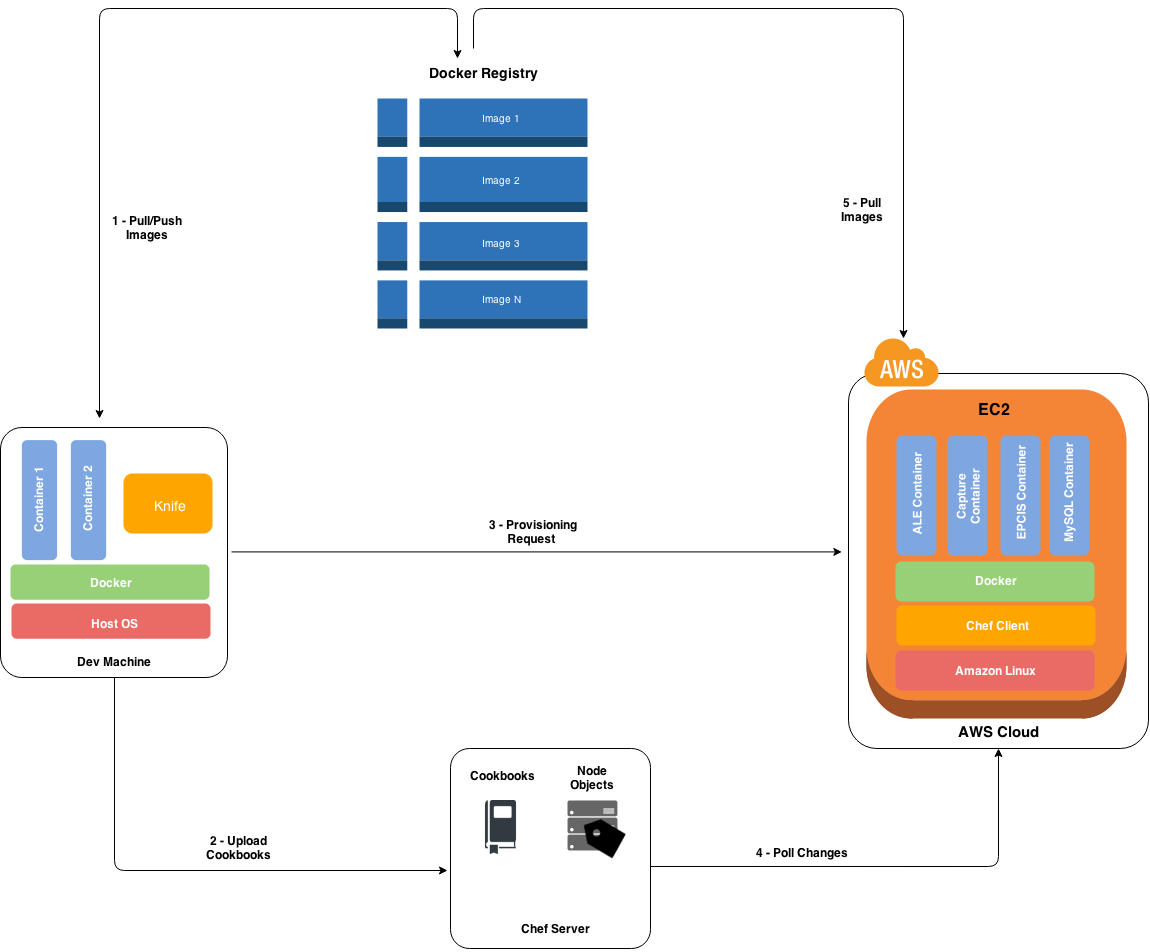
\includegraphics[width=\textwidth]{images/docker-c4t}
  \caption{Automatic provisioning workflow.}
  \label{fig:automatic_provisioning}
\end{figure}

In a development environment the Docker images are built and then uploaded to the Docker Registry
repository (1). The provisioning of the cloud resources is described in the cookbooks that are uploaded
to the Chef server (2). The provisioning request (3) is performed using knife - knife has a plugin for EC2
that allows to describe the image type, the instance type and the policies that need to be applied on
each provisioned node. The Chef client runs the configuration recipes that are sent by the Chef server (4).
In our solution this configuration recipes describe that a our nodes must have a set of Docker containers
running on it. The Chef client pulls the Docker images from the remote repository, built the
containers based on those images and finally apply the configuration that is associated to each container.

% -------------------------------------------------------------------------------------------------
% Containers
% -------------------------------------------------------------------------------------------------
\subsubsection{Containers}
\label{subs:containers}
Docker\footnote{https://www.docker.com} is an open source project to pack, ship and run any application
as a lightweight container. Docker containers are \textit{hardware-agnostic} and \textit{platform-agnostic},
this means that these containers can run anywhere, from a laptop to a EC2 compute instance. Since that Docker
is based in Linux Containers (LXC), the virtualization is performed at operating-system level, different of
hypervisor-based solutions where the virtualization is performed at hardware-level. While the effect of both
types of virtualization are similar, the virtualization at the operating-system level provides significant
benefits compared to hypervisor-based solutions. Docker containers are small, they have basically zero
memory and CPU overhead, they also are completable portable between different virtualization environments.

In our solution, we are using Docker containers for provisioning the software stack of the Fosstrak platform.
A complete installation of the Fosstrak platform requires a compatible Java SDK, a full MySQL database and
a Apache Tomcat server. In order to improve the application scalability we are provisioning a single container
for each component of the Fosstrak platform, the EPCIS repository, the Capture application, the ALE server,
and also for the MySQL database, as illustrated on Figure \ref{fig:docker_stack}.

% Dockerized application stack
\begin{figure}[!h]
  \centering
  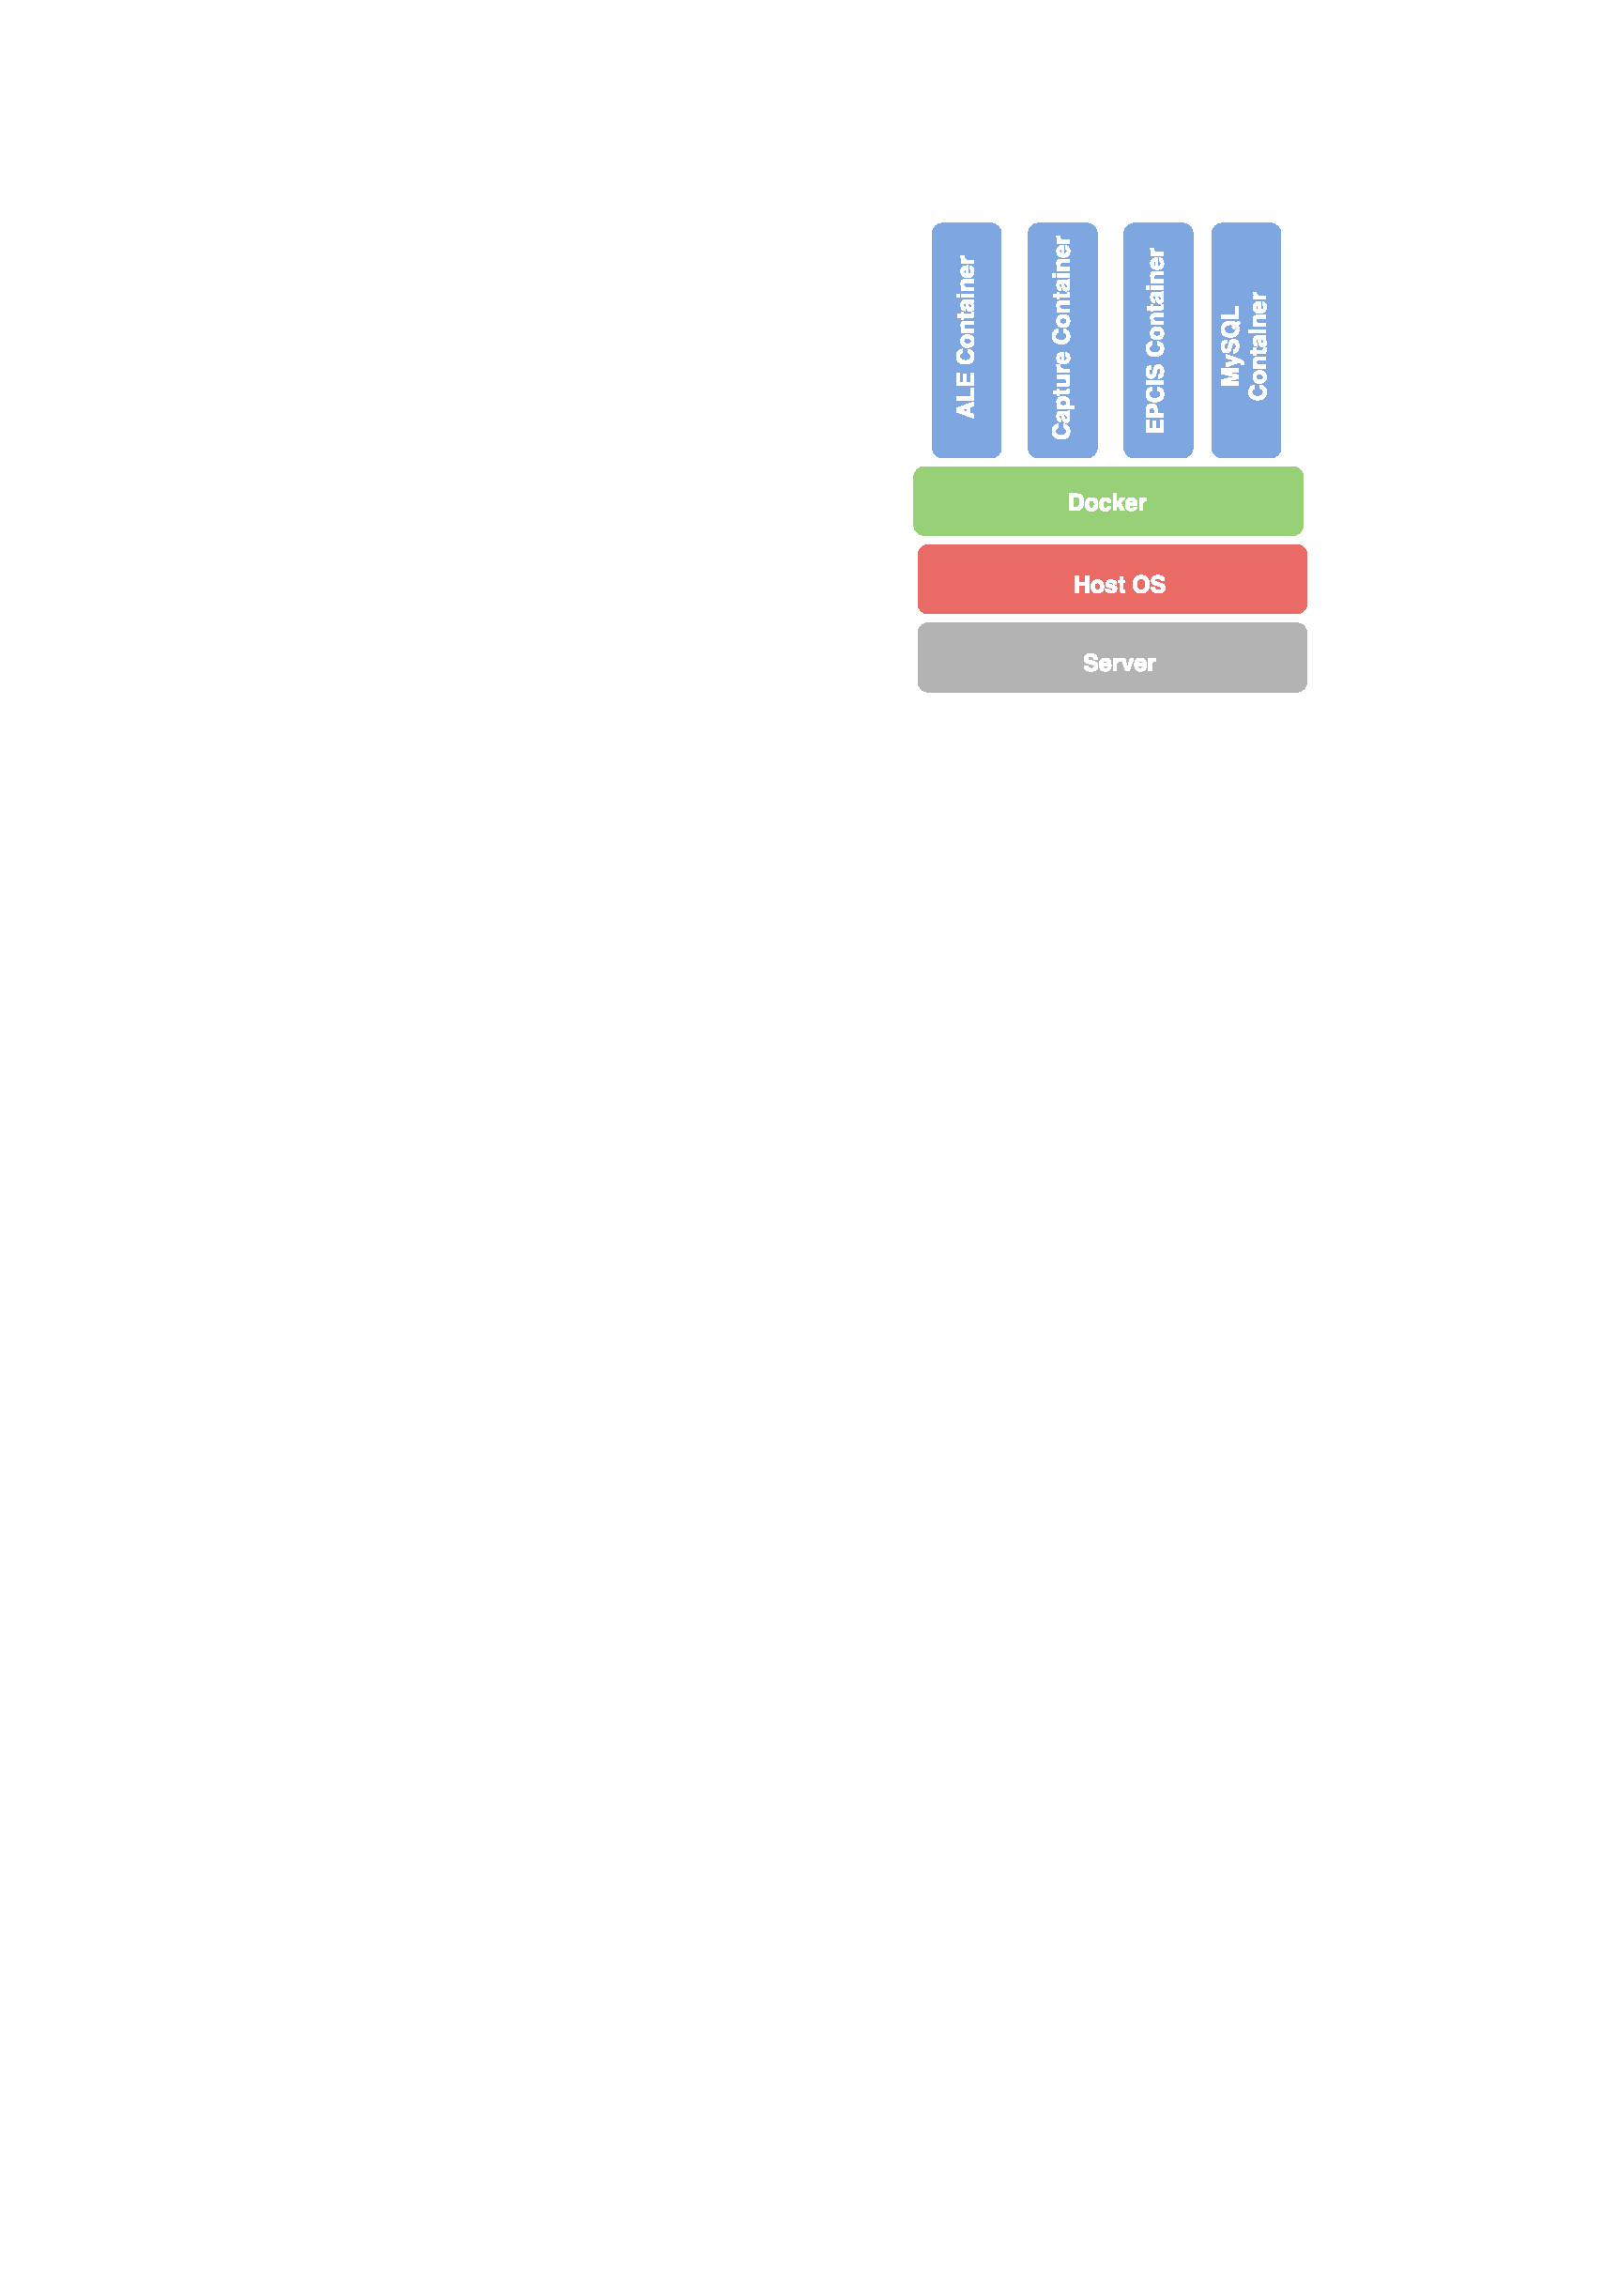
\includegraphics[width=.45\textwidth]{images/docker-stack}
  \caption{Container-based application stack.}
  \label{fig:docker_stack}
\end{figure}

By default each container runs a process that is isolated from the other processes that are executed in
the same machine. In order to connect the different modules of the Fosstrak platform, our containers are
linked through the \textit{linking} mechanism provided by Docker. Another benefit that the Docker platform
provides is the Docker Registry service, a public repository that stores Docker images used to create the
containers. In our solution we built the Docker images of the Fosstrak modules and publish them
in Docker registry to later be used to create our containers.
% -------------------------------------------------------------------------------------------------
% Configuration Management Tools
% -------------------------------------------------------------------------------------------------
\subsubsection{Configuration Management Tools}
\label{subs:cm_tools}
In our solution, the automatic provisioning of the infrastructure is performed through configuration
management tools, where for Cloud4Things we choose to use Chef\footnote{https://www.chef.io/}. Chef
allows to describe the infrastructure as code, in that way it is possible to automate how the
infrastructure is built, deployed and managed.

Chef architecture is composed of the Chef Server - that stores the recipes and other configuration data -
and the  Chef Client - that is installed in each server, VM or container, i.e, the nodes that are managed with Chef.
The Chef client periodically polls Chef server latest policy and state of the network, and if anything on the
node is out of date, the client update its state in order to be consistent with the latest policy.

Chef was built from the ground with the cloud infrastructure in mind. With Chef, is possible to dynamically
provision and de-provision the application infrastructure on demand to keep up with peaks in usage and traffic.
For instance, Chef offers several plugins for provisioning cloud resources in different hosts such as
Amazon EC2, Google Compute Engine and OpenStack.
